\documentclass[9pt,a4paper,oneside,hidelinks,aspectratio=169,dvipsnames]{beamer}
\usepackage[outputdir=build]{minted}
\usepackage[T1]{fontenc}
\usepackage[utf8]{inputenc}
\usepackage[english]{babel}
\usepackage{datetime}
\usepackage{lmodern}
\usepackage{graphicx}
\usepackage{csquotes}
\usepackage{amsmath}
\usepackage{caption}
\usepackage{subcaption}
\usepackage{pifont}
\usepackage{xspace}
\usepackage{pgfplots}
\usepackage{tikz}

\usetheme[progressbar=frametitle]{metropolis}
\setbeamerfont{block title}{size=\small}
\setbeamertemplate{section in toc}[sections numbered]
\captionsetup[figure]{font=tiny,labelsep=none}
\usetikzlibrary{automata, arrows.meta, shapes.geometric, calc, positioning, fit}

\newcommand{\cmark}{\ding{51}\xspace}%
\newcommand{\xmark}{\ding{55}\xspace}%
\newcommand{\code}[1]{\texttt{\detokenize{#1}}}
\newcommand{\codecpp}[1]{\mintinline[fontsize=\small]{C++}{#1}}

\title{Accelerating Halide on an FPGA by using CIRCT and Calyx as an intermediate step to go from a high-level and software-centric IRs down to RTL}
\date{May 15, 2023}
\author{Sergi Granell Escalfet}
\institute[Facultat d’Informàtica de Barcelona] {
  Master Degree in Innovation and Research in Informatics - High Performance Computing \\
  Facultat d’Informàtica de Barcelona \\
  Universitat Politècnica de Catalunya - BarcelonaTech
}

\pgfdeclareimage[height=0.6cm]{university-logo}{img/logo-upc-fib.png}
%\logo{\pgfputat{\pgfxy(-1.4,-1.0)}{\pgfbox[center,base]{\pgfuseimage{university-logo}}}}

\begin{document}

\maketitle

\begin{frame}
  \frametitle{Table of Contents}
  \tableofcontents
\end{frame}

\section{Introduction}

\begin{frame}{Image and array processing}
  \begin{itemize}
    \item Image processing and array processing play an essential role in modern life:
          \begin{itemize}
            \item Applying filters to the images that we upload to social media
            \item Running object detection algorithms on self-driving cars
          \end{itemize}
    \item $\uparrow$ \textbf{Sophistication} modern image processing pipelines, resolution image sensors, real-time video processing $\implies$ $\uparrow$ demand for highly \textbf{efficient} image processing pipeline implementations
    \item \textbf{Diversity} of targets: from a small device such as a smartphone, smartwatch or edge device to large data center and HPC systems
    \item Optimizing these algorithms can be \textbf{complex} and often results in \textbf{non-portable code}
          \begin{itemize}
            \item Hand-tuned C and assembly for a specific architecture
            \item Implementations optimized for an x86 multicore and a modern GPU have little resemblance
          \end{itemize}
  \end{itemize}
\end{frame}

\begin{frame}{Domain Specific Languages (DSLs)}
  \begin{itemize}
    \item DSLs: programming languages specialized to a \textbf{particular application domain}
    \item \textbf{Abstraction}: they provide a higher level of abstraction tailored to the specific domain
          \begin{itemize}
            \item Making it easier for developers to express complex concepts and ideas in a concise and natural way
          \end{itemize}
    \item \textbf{Expressiveness}: by focusing on a specific domain, DSLs enable developers to express their intent more directly, resulting in more readable and maintainable code
    \item \textbf{Productivity}: they simplify the development process. Focus on solving domain-specific problems rather than low-level implementation details
    \item \textbf{Performance}: they can be optimized for the specific domain, potentially allowing more efficient execution and better performance
    \item For the image/array processing application domain $\implies$ \textbf{Halide}
  \end{itemize}
\end{frame}

\section{Halide}

\begin{frame}[fragile]{Halide}
  \begin{itemize}
    \item Main idea: \textbf{decouple} the \textcolor{blue}{\textbf{\textit{algorithm}}} (\textquote{what needs to be computed}) definition from its \textcolor{blue}{\textbf{\textit{schedule}}} (\textquote{how it should be computed})
    \item W/o changing algorithm, explore different optimizations strategies (loop nesting and loop fusion, tiling, recomputation and storage balancing, vectorization, parallelism, \ldots)
  \end{itemize}
  \begin{figure}[H]
    \centering
    \begin{minipage}{\textwidth}
      \centering
      \begin{subfigure}[H]{.4\textwidth}
        \inputminted[tabsize=2,frame=single,rulecolor=gray,fontsize=\fontsize{4.2}{3}]{cpp}{fig/halide_manual_opt.cpp}
        \caption*{Hand-optimized C\texttt{++}. $x11$ faster. 0.9 ms/megapixel.}
      \end{subfigure}
      $\implies$
      \begin{subfigure}[H]{.4\textwidth}
        \inputminted[escapeinside=||,tabsize=2,frame=single,rulecolor=gray,fontsize=\fontsize{4.2}{3}]{cpp}{fig/halide_blur_3x3.cpp}
        \caption*{0.9 ms/megapixel.}
      \end{subfigure}
    \end{minipage}
  \end{figure}
\end{frame}

\begin{frame}[fragile]{Scheduling trade-offs (1)}
  \fontsize{6pt}{7.2}\selectfont
  \begin{figure}[H]
    \begin{minipage}{0.325\textwidth}
      \centering
      Blur 3x3 filter algorithm
      \centering
      \inputminted[tabsize=2,frame=single,rulecolor=gray,fontsize=\fontsize{5}{5}]{cpp}{fig/blur_3x3_base.cpp}
    \end{minipage}
  \end{figure}
  %\vspace{-0.5cm}
  \begin{figure}[H]
    \makebox[\linewidth]{
      \begin{minipage}{1.2\textwidth}
        \centering
        \begin{subfigure}[H]{.275\textwidth}
          \centering
          Breadth-first strategy
          \inputminted[tabsize=2,frame=single,rulecolor=gray,fontsize=\fontsize{4.2}{3}]{cpp}{fig/blur_3x3_breadth_first.cpp}
          \centering
          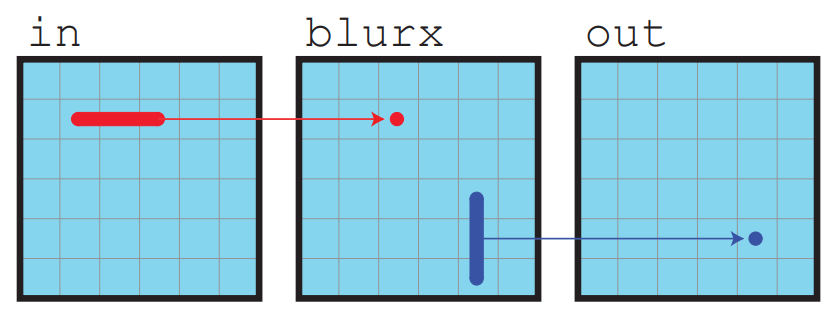
\includegraphics[width=3cm]{img/halide-breadth-first.png}
          \begin{itemize}
            \item[\xmark\xmark] Producer-consumer locality
            \item[\cmark\cmark] Parallelization
            \item[\cmark\cmark] Recomputation
          \end{itemize}
        \end{subfigure}
        \begin{subfigure}[H]{.31\textwidth}
          \centering
          Total fusion/inline strategy
          \inputminted[tabsize=2,frame=single,rulecolor=gray,fontsize=\fontsize{4.2}{3}]{cpp}{fig/blur_3x3_total_fusion.cpp}
          \vspace{0.3cm}
          \centering
          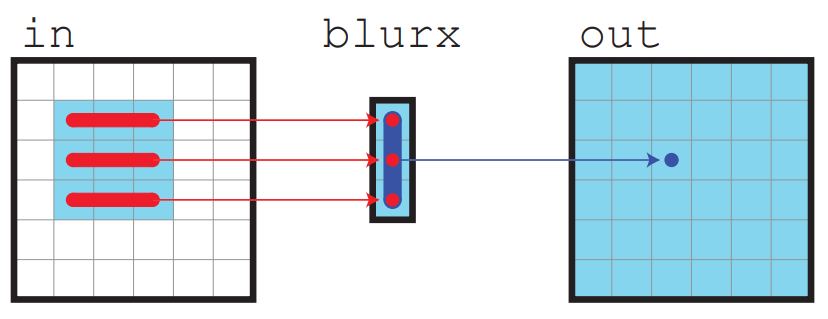
\includegraphics[width=3cm]{img/halide-total-fusion.png}
          \begin{itemize}
            \item[\cmark\cmark] Producer-consumer locality
            \item[\cmark\cmark] Parallelization
            \item[\xmark\xmark] Recomputation
          \end{itemize}
        \end{subfigure}
        \begin{subfigure}[H]{.3475\textwidth}
          \centering
          Sliding window strategy
          \inputminted[tabsize=2,frame=single,rulecolor=gray,fontsize=\fontsize{4.2}{3}]{cpp}{fig/blur_3x3_sliding_window.cpp}
          \centering
          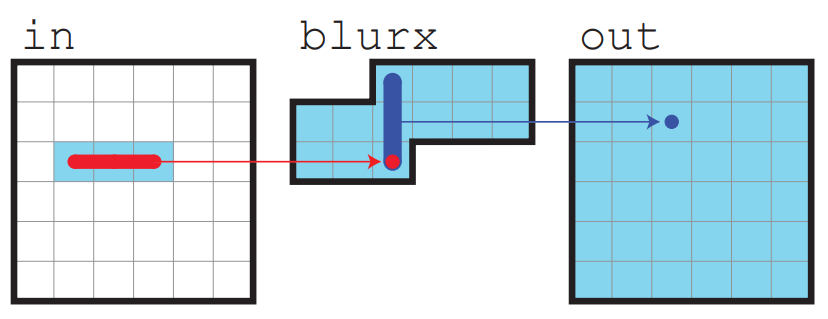
\includegraphics[width=3cm]{img/halide-sliding-window.png}
          \begin{itemize}
            \item[\cmark] Producer-consumer locality
            \item[\xmark\xmark] Parallelization
            \item[\cmark\cmark] Recomputation
          \end{itemize}
        \end{subfigure}
      \end{minipage}
    }
    \centering
    \unskip
    \vspace{0.3cm}
    \begin{tikzpicture}
      \coordinate (a) at (0cm,0cm);
      \coordinate (b) at (1.5cm,0);
      \coordinate (c) at (60:1.5cm);
      %
      \draw[color=black, fill=gray!40] (a) -- (b) -- (c) -- cycle;
      %
      \node[right = 0.1cm of b] {redundant work};
      \node[left = 0.1cm of a] {locality};
      \node[above = 0.1cm of c] {parallelism};
      \node[align=center] at (0.75cm, 0.4cm) {\tiny tradeoff\\\tiny space};
    \end{tikzpicture}
  \end{figure}
\end{frame}

\begin{frame}[fragile]{Scheduling trade-offs (2)}
  \fontsize{6pt}{7.2}\selectfont
  \vspace{0.25cm}
  \begin{figure}[H]
    \makebox[\linewidth]{
      \begin{minipage}{\textwidth}
        \centering
        \begin{subfigure}[H]{.45\textwidth}
          \centering
          Tiling strategy
          \inputminted[tabsize=2,frame=single,rulecolor=gray,fontsize=\fontsize{4.2}{3}]{cpp}{fig/blur_3x3_tiling.cpp}
          \centering
          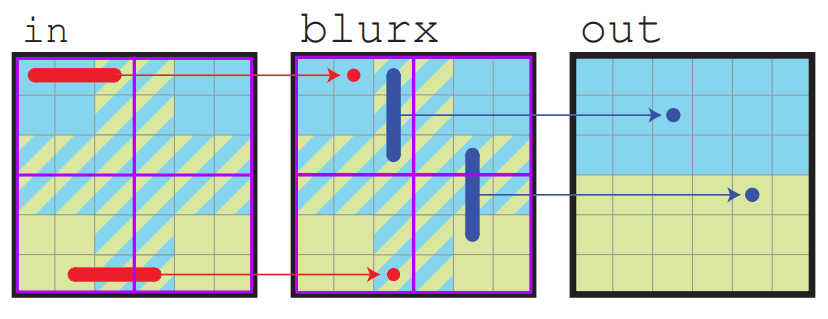
\includegraphics[width=3cm]{img/halide-tiling.png}
          \begin{itemize}
            \item[\cmark] Producer-consumer locality
            \item[\cmark\cmark] Parallelization
            \item[\xmark] Recomputation
          \end{itemize}
        \end{subfigure}
        \begin{subfigure}[H]{.45\textwidth}
          \centering
          Sliding window within tiling strategy
          \inputminted[tabsize=2,frame=single,rulecolor=gray,fontsize=\fontsize{4.2}{3}]{cpp}{fig/blur_3x3_sliding_window_tiling.cpp}
          \vspace{0.4cm}
          \centering
          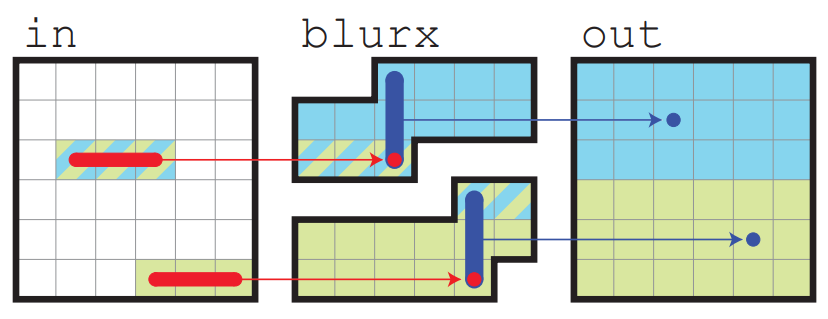
\includegraphics[width=3cm]{img/halide-sliding-window-tiling.png}
          \begin{itemize}
            \item[\cmark] Producer-consumer locality
            \item[\cmark] Parallelization
            \item[\cmark] Recomputation
          \end{itemize}
        \end{subfigure}
      \end{minipage}
    }
  \end{figure}
  \vspace{0.75cm}
  \metroset{block=fill}
  \begin{exampleblock}{Note}
    The best scheduling choice differs depending on each target architecture and the computational characteristics of the image pipeline stages.
  \end{exampleblock}
\end{frame}

\begin{frame}{Halide scheduling example}
  \fontsize{6pt}{7.2}\selectfont
  \begin{enumerate}
    \item Function's \textit{domain} is \textit{tiled} into $64\times64$-sized tiles
    \item Outer two loops of \textit{tiling} are \textit{fused} together into a single loop (\code{tile_index})
    \item \textit{Fused} loop is \textit{parallelized}
    \item Each \textit{tile} is \textit{tiled} again with $4\times2$-sized sub-tiles
    \item Sub-tile innermost $x$-loop (\code{x_vectors}) is \textit{vectorized} with the same factor as \code{x_vectors} ($4$): no iterations will be performed at this nesting level, the whole loop will be vectorized
    \item Sub-tile $y$-loop (\code{y_pairs}) is fully \textit{unrolled} with a factor matching the sub-tile vertical size ($2$), therefore eliminating the sub-tile inner loops in favor of \textit{unrolling} and \textit{vectorization}
  \end{enumerate}

  \begin{figure}[H]
    \begin{minipage}{0.6\textwidth}
      \centering
      \inputminted[tabsize=2,frame=single,rulecolor=gray,fontsize=\fontsize{5}{5}]{cpp}{fig/halide_scheduling_example.cpp}
    \end{minipage}
  \end{figure}
\end{frame}

\begin{frame}{Halide compilation flow}
  \fontsize{6pt}{7.2}\selectfont
  \begin{enumerate}
    \item \textbf{Lowering and loop synthesis}: given the \textit{schedule}, it generates the loop nests and allocations required to evaluate the pipeline, beginning from the output.
    \item \textbf{Bounds inference}: recursively back from the output and using interval analysis, for each function, it evaluates the bounds of the dimensions based on the bounds required by its caller and the indices it is called with.
    \item \textbf{Sliding window optimization and storage folding}: traverses the loop nests seeking opportunities for sliding window optimizations (when the results of a function are to be stored by a serial loop at a higher loop nesting level than its computation).
    \item \textbf{Flattening}: multi-dimensional loads, stores, and allocations are flattened into their linear single-dimensional equivalent.
    \item \textbf{Vectorization and unrolling}: converts loops that were scheduled as vectorized or unrolled into the corresponding loops. During vectorization, occurrences of a loop index are replaced with a special value $ramp(n)$ which represents the vector $[0, 1, \ldots, n-1]$.
    \item \textbf{Back-end code generation}: low-level optimizations are performed and machine code is emitted for the resulting pipeline. The primary backends use LLVM for code generation. After running constant-folding and dead-code elimination passes the Halide IR, it is ready to be lowered (\code{CodeGen} backend).
  \end{enumerate}

  \begin{figure}[H]
    \centering
    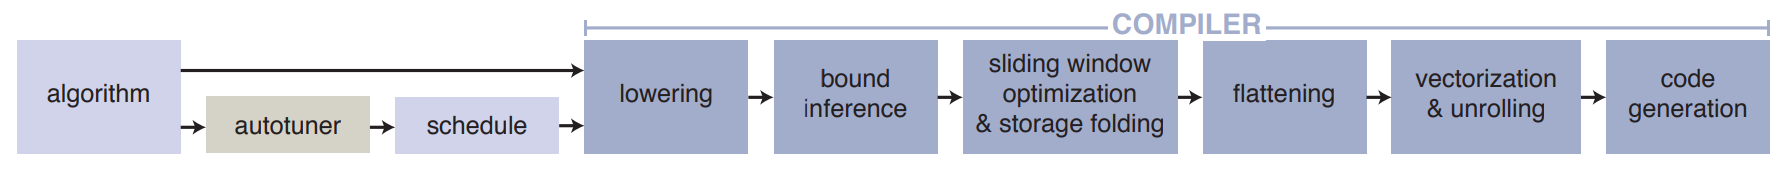
\includegraphics[width=\textwidth]{img/halide-compiler-flow.png}
  \end{figure}

\end{frame}

\begin{frame}{Halide IR}
  \fontsize{6pt}{7.2}\selectfont


\end{frame}

\end{document}
